\documentclass[]{book}
\usepackage{lmodern}
\usepackage{amssymb,amsmath}
\usepackage{ifxetex,ifluatex}
\usepackage{fixltx2e} % provides \textsubscript
\ifnum 0\ifxetex 1\fi\ifluatex 1\fi=0 % if pdftex
  \usepackage[T1]{fontenc}
  \usepackage[utf8]{inputenc}
\else % if luatex or xelatex
  \ifxetex
    \usepackage{mathspec}
  \else
    \usepackage{fontspec}
  \fi
  \defaultfontfeatures{Ligatures=TeX,Scale=MatchLowercase}
\fi
% use upquote if available, for straight quotes in verbatim environments
\IfFileExists{upquote.sty}{\usepackage{upquote}}{}
% use microtype if available
\IfFileExists{microtype.sty}{%
\usepackage{microtype}
\UseMicrotypeSet[protrusion]{basicmath} % disable protrusion for tt fonts
}{}
\usepackage[margin=1in]{geometry}
\usepackage{hyperref}
\hypersetup{unicode=true,
            pdftitle={Medidas de Alpha Diversidad},
            pdfauthor={Carlos Iván Espinosa},
            pdfborder={0 0 0},
            breaklinks=true}
\urlstyle{same}  % don't use monospace font for urls
\usepackage{natbib}
\bibliographystyle{apalike}
\usepackage{color}
\usepackage{fancyvrb}
\newcommand{\VerbBar}{|}
\newcommand{\VERB}{\Verb[commandchars=\\\{\}]}
\DefineVerbatimEnvironment{Highlighting}{Verbatim}{commandchars=\\\{\}}
% Add ',fontsize=\small' for more characters per line
\usepackage{framed}
\definecolor{shadecolor}{RGB}{248,248,248}
\newenvironment{Shaded}{\begin{snugshade}}{\end{snugshade}}
\newcommand{\KeywordTok}[1]{\textcolor[rgb]{0.13,0.29,0.53}{\textbf{{#1}}}}
\newcommand{\DataTypeTok}[1]{\textcolor[rgb]{0.13,0.29,0.53}{{#1}}}
\newcommand{\DecValTok}[1]{\textcolor[rgb]{0.00,0.00,0.81}{{#1}}}
\newcommand{\BaseNTok}[1]{\textcolor[rgb]{0.00,0.00,0.81}{{#1}}}
\newcommand{\FloatTok}[1]{\textcolor[rgb]{0.00,0.00,0.81}{{#1}}}
\newcommand{\ConstantTok}[1]{\textcolor[rgb]{0.00,0.00,0.00}{{#1}}}
\newcommand{\CharTok}[1]{\textcolor[rgb]{0.31,0.60,0.02}{{#1}}}
\newcommand{\SpecialCharTok}[1]{\textcolor[rgb]{0.00,0.00,0.00}{{#1}}}
\newcommand{\StringTok}[1]{\textcolor[rgb]{0.31,0.60,0.02}{{#1}}}
\newcommand{\VerbatimStringTok}[1]{\textcolor[rgb]{0.31,0.60,0.02}{{#1}}}
\newcommand{\SpecialStringTok}[1]{\textcolor[rgb]{0.31,0.60,0.02}{{#1}}}
\newcommand{\ImportTok}[1]{{#1}}
\newcommand{\CommentTok}[1]{\textcolor[rgb]{0.56,0.35,0.01}{\textit{{#1}}}}
\newcommand{\DocumentationTok}[1]{\textcolor[rgb]{0.56,0.35,0.01}{\textbf{\textit{{#1}}}}}
\newcommand{\AnnotationTok}[1]{\textcolor[rgb]{0.56,0.35,0.01}{\textbf{\textit{{#1}}}}}
\newcommand{\CommentVarTok}[1]{\textcolor[rgb]{0.56,0.35,0.01}{\textbf{\textit{{#1}}}}}
\newcommand{\OtherTok}[1]{\textcolor[rgb]{0.56,0.35,0.01}{{#1}}}
\newcommand{\FunctionTok}[1]{\textcolor[rgb]{0.00,0.00,0.00}{{#1}}}
\newcommand{\VariableTok}[1]{\textcolor[rgb]{0.00,0.00,0.00}{{#1}}}
\newcommand{\ControlFlowTok}[1]{\textcolor[rgb]{0.13,0.29,0.53}{\textbf{{#1}}}}
\newcommand{\OperatorTok}[1]{\textcolor[rgb]{0.81,0.36,0.00}{\textbf{{#1}}}}
\newcommand{\BuiltInTok}[1]{{#1}}
\newcommand{\ExtensionTok}[1]{{#1}}
\newcommand{\PreprocessorTok}[1]{\textcolor[rgb]{0.56,0.35,0.01}{\textit{{#1}}}}
\newcommand{\AttributeTok}[1]{\textcolor[rgb]{0.77,0.63,0.00}{{#1}}}
\newcommand{\RegionMarkerTok}[1]{{#1}}
\newcommand{\InformationTok}[1]{\textcolor[rgb]{0.56,0.35,0.01}{\textbf{\textit{{#1}}}}}
\newcommand{\WarningTok}[1]{\textcolor[rgb]{0.56,0.35,0.01}{\textbf{\textit{{#1}}}}}
\newcommand{\AlertTok}[1]{\textcolor[rgb]{0.94,0.16,0.16}{{#1}}}
\newcommand{\ErrorTok}[1]{\textcolor[rgb]{0.64,0.00,0.00}{\textbf{{#1}}}}
\newcommand{\NormalTok}[1]{{#1}}
\usepackage{longtable,booktabs}
\usepackage{graphicx,grffile}
\makeatletter
\def\maxwidth{\ifdim\Gin@nat@width>\linewidth\linewidth\else\Gin@nat@width\fi}
\def\maxheight{\ifdim\Gin@nat@height>\textheight\textheight\else\Gin@nat@height\fi}
\makeatother
% Scale images if necessary, so that they will not overflow the page
% margins by default, and it is still possible to overwrite the defaults
% using explicit options in \includegraphics[width, height, ...]{}
\setkeys{Gin}{width=\maxwidth,height=\maxheight,keepaspectratio}
\IfFileExists{parskip.sty}{%
\usepackage{parskip}
}{% else
\setlength{\parindent}{0pt}
\setlength{\parskip}{6pt plus 2pt minus 1pt}
}
\setlength{\emergencystretch}{3em}  % prevent overfull lines
\providecommand{\tightlist}{%
  \setlength{\itemsep}{0pt}\setlength{\parskip}{0pt}}
\setcounter{secnumdepth}{5}
% Redefines (sub)paragraphs to behave more like sections
\ifx\paragraph\undefined\else
\let\oldparagraph\paragraph
\renewcommand{\paragraph}[1]{\oldparagraph{#1}\mbox{}}
\fi
\ifx\subparagraph\undefined\else
\let\oldsubparagraph\subparagraph
\renewcommand{\subparagraph}[1]{\oldsubparagraph{#1}\mbox{}}
\fi

%%% Use protect on footnotes to avoid problems with footnotes in titles
\let\rmarkdownfootnote\footnote%
\def\footnote{\protect\rmarkdownfootnote}

%%% Change title format to be more compact
\usepackage{titling}

% Create subtitle command for use in maketitle
\newcommand{\subtitle}[1]{
  \posttitle{
    \begin{center}\large#1\end{center}
    }
}

\setlength{\droptitle}{-2em}
  \title{Medidas de Alpha Diversidad}
  \pretitle{\vspace{\droptitle}\centering\huge}
  \posttitle{\par}
  \author{Carlos Iván Espinosa}
  \preauthor{\centering\large\emph}
  \postauthor{\par}
  \predate{\centering\large\emph}
  \postdate{\par}
  \date{Octubre de 2016}

\usepackage{booktabs}

\begin{document}
\maketitle

{
\setcounter{tocdepth}{1}
\tableofcontents
}
\chapter*{Preambulo}\label{preambulo}
\addcontentsline{toc}{chapter}{Preambulo}

A partir de la composición de especies de las comunidades naturales
podemos extraer medidas que nos permite simplificar los datos de la
comunidad obteniendo algunas de sus propiedades emergentes.

Las comunidades cambian a lo largo del paisaje como una respuesta a las
variaciones del ambiente, estos cambios en el paisaje han hecho
necesario el separar los componentes de la diversidad de la comunidad.
Según Whittaker (1972) podemos separar la diversidad en los componentes
\emph{alfa, beta} y \emph{gamma}. La diversidad \emph{\textbf{alfa}} se
refiere a la riqueza de especies que detectamos en una comunidad en un
determinado sitio más o menos homogéneo. La diversidad
\emph{\textbf{beta}} se refiere al grado de cambio o reemplazo de
especies entre diferentes comunidades en un paisaje, y la diversidad
\emph{\textbf{gamma}} se refiere a la riqueza de especies del conjunto
de comunidades que integran un paisaje y es el resultado de las
diversidades alfa y beta en el territorio (Whittaker, 1972).

\begin{quote}
La diversidad puede ser separada en diversidad alfa, beta y gamma

--- (Wittaker, 1972)
\end{quote}

La diversidad alfa está constituida por la diversidad intrínseca de una
comunidad bajo condiciones similares en un paisaje. Existen tres medidas
de alfa diversidad; riqueza, equitatividad y diversidad.

La riqueza, posiblemente la medida más sencilla, se refiere al número de
especies en un determinado sitio independiente de las abundancias de
cada una. Aunque la riqueza y los índices basados en esta son
interesantes perdemos una parte de la información en estos índices, la
abundancia.

La equitatividad se refiere a la variabilidad en las abundancias
relativas de cada una de las especies de la comunidad. Es una medida que
nos permite entender el reparto de recursos entre las especies dentro de
la comunidad, y por tanto cual es el aporte de cada una de las especies
a la comunidad.

Los índices de diversidad están basados en la relación entre
equitatividad y riqueza. Aunque hay más de 60 índices publicados en
revistas ecológicas los índices de Shannon-Weaver y de Simpson son los
más comunes para medir alfa diversidad. La meta fundamental detrás del
diseño de la mayoría de los índices de diversidad es unificar dos
elementos de la diversidad, la equitatividad, o sea la variabilidad en
las abundancias relativas de las especies de la comunidad, y la riqueza,
o sea el número total de especies que componen la comunidad.


\includegraphics{Alpha-Diversidad_files/figure-latex/unnamed-chunk-1-1.pdf}

\chapter{Objetivos}\label{objetivos}

\begin{itemize}
\tightlist
\item
  Comprender los factores que influencian la riqueza y diversidad de
  especies.
\end{itemize}

\begin{itemize}
\tightlist
\item
  Comprender los métodos para medir y describir la riqueza y diversidad
  de las comunidades y su aplicación en el contexto de campo.
\end{itemize}

\chapter{Riqueza total del muestreo}\label{riqueza-total-del-muestreo}

La riqueza es definida como el número de especies que habitan en una
comunidad espacial y temporalmente homogénea. Posiblemente es la forma
más directa y clara de medir la diversidad biológica (Sarkar, 2002;
Magurran, 2004). Sin embargo, medir la riqueza de forma precisa no es
una tarea sencilla (Magurran, 2004), debido a que el número de especies
observadas aumenta con el esfuerzo de muestreo. Por ello, la riqueza
debería determinarse sólo a partir de inventarios completos, lo que
generalmente es poco práctico o muy difícil de lograr (González-Oreja et
al. 2010).

Pero \emph{¿qué es un inventario completo? ¿Cómo puedo saber si mi
inventario ha sido lo suficientemente bueno como para registrar todas
las especies?}. Una manera de evaluar si el esfuerzo de muestreo ha sido
exitoso es la curva de acumulación de especies. Los modelos de
acumulación de especies estudian la acumulación de especies cuando el
número de sitios aumenta. Hay varios métodos alternativos, incluyendo la
acumulación de los sitios en el orden en que se encuentren, y la
acumulación repetida en orden aleatorio (Oksanen, 2015).

Vamos a analizar cómo construir estas curvas.

\begin{Shaded}
\begin{Highlighting}[]
\KeywordTok{library}\NormalTok{(vegan)}
\KeywordTok{data}\NormalTok{(BCI)}
\KeywordTok{set.seed}\NormalTok{(}\DecValTok{6}\NormalTok{)}
\CommentTok{#Obtenemos una submuestra de BCI}
\NormalTok{BCI_sub <-}\StringTok{ }\NormalTok{BCI[}\KeywordTok{c}\NormalTok{(}\KeywordTok{sample}\NormalTok{(}\DecValTok{1}\NormalTok{:}\DecValTok{50}\NormalTok{, }\DecValTok{10}\NormalTok{, }\DataTypeTok{replace =} \OtherTok{TRUE}\NormalTok{)),]}
\NormalTok{BCI_sub <-}\StringTok{ }\NormalTok{BCI_sub[,}\KeywordTok{colSums}\NormalTok{(BCI_sub)>=}\DecValTok{1} \NormalTok{] }
\CommentTok{#Eliminamos las especies sin datos}
\end{Highlighting}
\end{Shaded}

Ahora realizamos la curva de acumulación de especies por parcelas.
Utilizamos la función \texttt{specaccum} del paquete vegan, el argumento
\emph{method} permite generar una curva con orden impuesto por el
colector.

\begin{Shaded}
\begin{Highlighting}[]
\NormalTok{col<-}\KeywordTok{specaccum}\NormalTok{(BCI_sub, }\DataTypeTok{method =} \StringTok{"collector"}\NormalTok{)}
\KeywordTok{plot}\NormalTok{(col, }\DataTypeTok{xlab=}\StringTok{"Parcelas"}\NormalTok{, }\DataTypeTok{ylab=}\StringTok{"Número de especies"}\NormalTok{, }\DataTypeTok{col=}\StringTok{"blue"}\NormalTok{)}
\KeywordTok{points}\NormalTok{(col$richness, }\DataTypeTok{pch=}\DecValTok{19}\NormalTok{, }\DataTypeTok{col=}\StringTok{"darkblue"}\NormalTok{)}
\end{Highlighting}
\end{Shaded}

\begin{figure}

{\centering 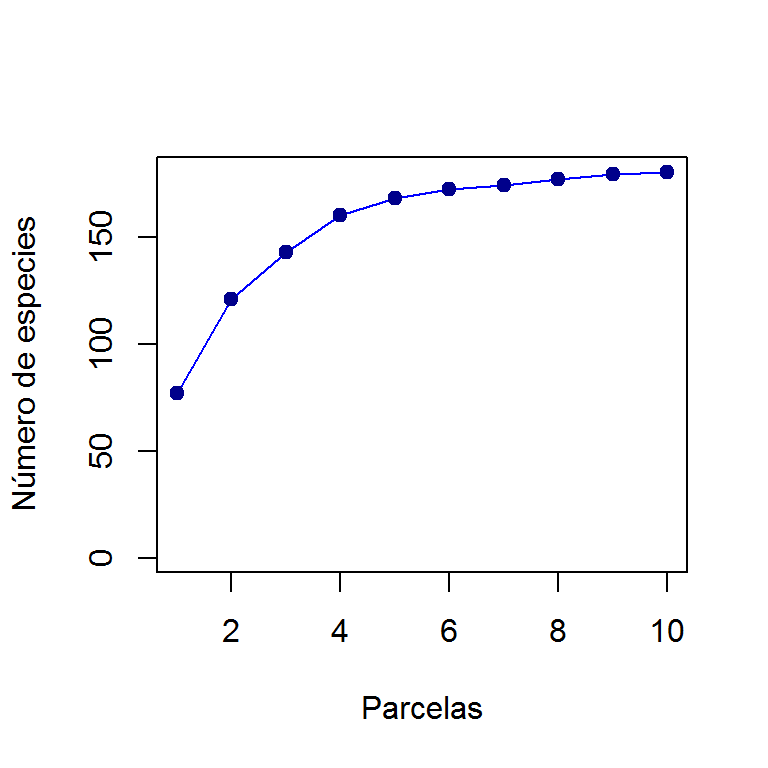
\includegraphics{Alpha-Diversidad_files/figure-latex/accum-1} 

}

\caption{Curva de acumulación de especies}\label{fig:accum}
\end{figure}

En la figura \ref{fig:accum} podemos ver como las nuevas especies van
incrementando la riqueza con el aumento del área muestreal, la curva
muestra ``saltos'' cuando sumamos las especies nuevas de cada nueva
parcela. La aparición de las especies es definida por el colector, en
otras palabras es tal y como hemos subido los datos.

Estas curvas son utilizadas para evaluar el esfuerzo de muestreo. Se
cree que si el muestreo ha llegado a su asíntota (ya no hay más ingresos
a la riqueza de especies) entonces el muestreo es suficiente.

\chapter{Rarefacción}\label{rarefaccion}

La riqueza es una de las medidas más simples e intuitivas que describen
una comunidad, sin embargo, uno de los problemas del uso de esta medida
es su dependencia del tamaño muestreal (Magurran 2004), esto implica que
la riqueza (y las otras medidas de diversidad) puede verse influida por
variaciones en el esfuerzo muestreal. Aunque el diseño experimental está
pensado para estandarizar el esfuerzo muestreal, los tamaños finales
muestreales difícilmente son iguales.

\begin{quote}
Un esfuerzo de muestreo desigual puede tener impactos en las medidas de
riqueza de especies

--- (Magurran 2004)
\end{quote}

Esto representa un inconveniente, ya que muestreos en principio del
mismo tamaño, podrían capturar números significativamente diferentes de
individuos. Pensemos que una red para aves podría capturar 150
individuos en un sitio y 25 en otro. Cuan comparables serían estos datos
si sabemos que el tamaño de la muestra influye en la cantidad de
especies colectadas.

De esta manera, necesitamos separar dos conceptos distintos, la densidad
de especies de la riqueza de especies. Imaginemos dos área cualquiera
donde vamos a muestrear la vegetación, estas dos áreas únicamente se
diferencian porque en la una existe pastoreo y en la otra no. Vemos que
pasa cuando muestreamos cada una de estas comunidades.

\begin{Shaded}
\begin{Highlighting}[]
\CommentTok{#Generamos unas comunidades}
\NormalTok{pas <-}\StringTok{ }\KeywordTok{data.frame}\NormalTok{( }\DataTypeTok{sp =} \KeywordTok{paste}\NormalTok{(}\KeywordTok{rep}\NormalTok{(}\StringTok{"sp"}\NormalTok{, }\DecValTok{30}\NormalTok{), }\DecValTok{1}\NormalTok{:}\DecValTok{30}\NormalTok{, }\DataTypeTok{sep=}\StringTok{"-"}\NormalTok{), }\DataTypeTok{abun=} \KeywordTok{sample}\NormalTok{(}\DecValTok{1}\NormalTok{:}\DecValTok{12}\NormalTok{, }\DecValTok{30}\NormalTok{, }\DataTypeTok{replace=}\OtherTok{TRUE}\NormalTok{))}
\NormalTok{pas1 <-}\StringTok{ }\KeywordTok{matrix}\NormalTok{(}\DecValTok{0}\NormalTok{, }\DecValTok{40}\NormalTok{,}\DecValTok{30}\NormalTok{)}
\KeywordTok{colnames}\NormalTok{(pas1) <-}\StringTok{ }\NormalTok{pas[,}\DecValTok{1}\NormalTok{]}
\NormalTok{for(i in }\DecValTok{1}\NormalTok{:}\DecValTok{30}\NormalTok{)\{}
\NormalTok{pas1[,i] <-}\StringTok{ }\KeywordTok{c}\NormalTok{(}\KeywordTok{rep}\NormalTok{(}\DecValTok{1}\NormalTok{, pas[i,}\DecValTok{2}\NormalTok{]), }\KeywordTok{rep}\NormalTok{(}\DecValTok{0}\NormalTok{, }\DecValTok{40}\NormalTok{-pas[i,}\DecValTok{2}\NormalTok{]))}
\NormalTok{\}}
\NormalTok{pas1 <-}\StringTok{ }\NormalTok{pas1[}\KeywordTok{order}\NormalTok{(}\KeywordTok{sample}\NormalTok{(}\DecValTok{1}\NormalTok{:}\DecValTok{40}\NormalTok{, }\DecValTok{30}\NormalTok{)), ]}

\NormalTok{npas <-}\StringTok{ }\KeywordTok{data.frame}\NormalTok{( }\DataTypeTok{sp =} \KeywordTok{paste}\NormalTok{(}\KeywordTok{rep}\NormalTok{(}\StringTok{"sp"}\NormalTok{, }\DecValTok{30}\NormalTok{), }\DecValTok{1}\NormalTok{:}\DecValTok{30}\NormalTok{, }\DataTypeTok{sep=}\StringTok{"-"}\NormalTok{), }\DataTypeTok{abun=} \KeywordTok{sample}\NormalTok{(}\DecValTok{30}\NormalTok{:}\DecValTok{40}\NormalTok{, }\DecValTok{30}\NormalTok{, }\DataTypeTok{replace=}\OtherTok{TRUE}\NormalTok{))}
\NormalTok{npas1 <-}\StringTok{ }\KeywordTok{matrix}\NormalTok{(}\DecValTok{0}\NormalTok{, }\DecValTok{40}\NormalTok{,}\DecValTok{30}\NormalTok{)}
\KeywordTok{colnames}\NormalTok{(npas1) <-}\StringTok{ }\NormalTok{npas[,}\DecValTok{1}\NormalTok{]}
\NormalTok{for(i in }\DecValTok{1}\NormalTok{:}\DecValTok{30}\NormalTok{)\{}
\NormalTok{npas1[,i] <-}\StringTok{ }\KeywordTok{c}\NormalTok{(}\KeywordTok{rep}\NormalTok{(}\DecValTok{1}\NormalTok{, npas[i,}\DecValTok{2}\NormalTok{]), }\KeywordTok{rep}\NormalTok{(}\DecValTok{0}\NormalTok{, }\DecValTok{40}\NormalTok{-npas[i,}\DecValTok{2}\NormalTok{]))}
\NormalTok{\}}
\NormalTok{npas1 <-}\StringTok{ }\NormalTok{npas1[}\KeywordTok{order}\NormalTok{(}\KeywordTok{sample}\NormalTok{(}\DecValTok{1}\NormalTok{:}\DecValTok{20}\NormalTok{, }\DecValTok{20}\NormalTok{)), ]}

\CommentTok{#Ahora las muestreamos}
\NormalTok{m_pas <-}\StringTok{ }\KeywordTok{matrix}\NormalTok{(}\DecValTok{0}\NormalTok{,}\DecValTok{3}\NormalTok{,}\DecValTok{30}\NormalTok{)}
\KeywordTok{colnames}\NormalTok{(m_pas) <-}\StringTok{ }\KeywordTok{colnames}\NormalTok{(pas1)}
\NormalTok{m_pas[}\DecValTok{1}\NormalTok{,] <-}\StringTok{ }\KeywordTok{sample}\NormalTok{(pas1, }\DecValTok{30}\NormalTok{)}
\NormalTok{m_pas[}\DecValTok{2}\NormalTok{,] <-}\StringTok{ }\KeywordTok{sample}\NormalTok{(pas1, }\DecValTok{30}\NormalTok{)}
\NormalTok{m_pas[}\DecValTok{3}\NormalTok{,] <-}\StringTok{ }\KeywordTok{sample}\NormalTok{(pas1, }\DecValTok{30}\NormalTok{)}

\NormalTok{m_npas <-}\StringTok{ }\KeywordTok{matrix}\NormalTok{(}\DecValTok{0}\NormalTok{,}\DecValTok{3}\NormalTok{,}\DecValTok{30}\NormalTok{)}
\KeywordTok{colnames}\NormalTok{(m_npas) <-}\StringTok{ }\KeywordTok{colnames}\NormalTok{(pas1)}
\NormalTok{m_npas[}\DecValTok{1}\NormalTok{,] <-}\StringTok{ }\KeywordTok{sample}\NormalTok{(npas1, }\DecValTok{30}\NormalTok{)}
\NormalTok{m_npas[}\DecValTok{2}\NormalTok{,] <-}\StringTok{ }\KeywordTok{sample}\NormalTok{(npas1, }\DecValTok{30}\NormalTok{)}
\NormalTok{m_npas[}\DecValTok{3}\NormalTok{,] <-}\StringTok{ }\KeywordTok{sample}\NormalTok{(npas1, }\DecValTok{30}\NormalTok{)}

\CommentTok{#Calculamos la riqueza de las muestras}
\KeywordTok{specnumber}\NormalTok{(}\KeywordTok{colSums}\NormalTok{(m_pas)) }\CommentTok{#Pastoreado}
\end{Highlighting}
\end{Shaded}

\begin{verbatim}
## [1] 15
\end{verbatim}

\begin{Shaded}
\begin{Highlighting}[]
\KeywordTok{specnumber}\NormalTok{(}\KeywordTok{colSums}\NormalTok{(m_npas))}\CommentTok{#No Pastoreado}
\end{Highlighting}
\end{Shaded}

\begin{verbatim}
## [1] 30
\end{verbatim}

Como vemos por puro azar la diversidad es mucho mayor en las parcelas no
pastoreadas, pero realmente hay mayor diversidad? Obtengamos la
diversidad total de cada comunidad.

\begin{Shaded}
\begin{Highlighting}[]
\KeywordTok{specnumber}\NormalTok{(}\KeywordTok{colSums}\NormalTok{(pas1))}\CommentTok{#Pastoreado}
\end{Highlighting}
\end{Shaded}

\begin{verbatim}
## [1] 30
\end{verbatim}

\begin{Shaded}
\begin{Highlighting}[]
\KeywordTok{specnumber}\NormalTok{(}\KeywordTok{colSums}\NormalTok{(npas1))}\CommentTok{#No Pastoreado}
\end{Highlighting}
\end{Shaded}

\begin{verbatim}
## [1] 30
\end{verbatim}

Efectivamente la riqueza es la misma, el único problema es que en la
zona pastoreada tiene una menor abundancia lo que origina una menor
densidad de especies, sin embargo, no hay un efecto sobre la riqueza de
especies.

Algunos índices basados en la riqueza como el de Margalef y Menhinick
han sido propuestos para minimizar estos efectos, pero este ajuste ha
mostrado ser insuficiente (Magurran, 2004). Una solución más aceptada a
este problema es realizar una rarefacción, que es una forma de
remuestrear las parcelas en función de un tamaño de muestra único para
todas las parcelas.

Específicamente la rarefacción es el proceso de generación de la
relación entre el número de especies vs el número de individuos en una o
más muestras (Stevens 2009). Esta corrección por el número de individuos
nos permite la comparación directa de la riqueza de dos muestras que
inicialmente tenían diferente tamaño.

Para poder abordar estos temas utilizaremos la función \texttt{rarefy}
del paquete \emph{vegan}. La función \texttt{rarefy} arroja como
resultado la riqueza de especies esperada en un determinado tamaño de
muestra.

La rarefacción puede realizarse solamente con auténticos datos de
conteos. La función \emph{rarefy} se basa en la formulación de Hurlbert
(1971), y los errores estándar sobre Heck et al. (1975).

Hurlbert (1971) propone la rarefacción como:

\[S_n= \sum_{i=1}^S (1-q_i)\]

Donde; \(q_i= \frac{(\frac{n-x_i}{n})}{(\frac{N}{n})}\) que representa
las probabilidades de que las especies \emph{i} no ocurra en una muestra
de tamaño \emph{n}, \(x_i\) es el conteo de \emph{i} especies y
\((\frac{N}{n})\) es el coeficiente binomial o el número de formas en
las que puede elegir n de N

En otras palabras la rarefacción permite hacer una interpolación de los
datos, obteniendo una riqueza esperada en un tamaño de muestra menor al
tamaño que hemos logrado, de esta forma este proceso nos da no solamente
la riqueza sino un error estándar. Si la muestra es un vector, la
rarefacción se calculará para cada tamaño de la muestra por separado.

A continuación vamos a utilizar la función \emph{rarefy} para construir
las curvas de rarefacción basadas en individuos y en muestras.

\section{Rarefacción basada en
Individuos}\label{rarefaccion-basada-en-individuos}

Vamos a utilizar nuestros ya conocidos datos de BCI, a partir de estos
datos realizaremos un submuestreo escogiendo 10 de las 50 parcelas de
BCI, esto con el fin de simplificar el ejemplo.

Lo primero que necesitamos es obtener un vector (un objeto) con el total
de individuos de cada especie, este objeto representa la comunidad sobre
la que haremos la rarefacción y la estimación de la riqueza total.
Queremos generar una curva parecida a la de acumulación de especies pero
que nos dará una riqueza con el error estándar, para esto tenemos que
definir en qué tamaños de muestra queremos hacer la interpolación. Vamos
a realizar estos pasos en R.

\begin{Shaded}
\begin{Highlighting}[]
\CommentTok{#Usaremos los datos con los cuales construimos las curvas de acumulación}
\CommentTok{#Sumamos la abundancia de cada especie}
\NormalTok{N <-}\StringTok{ }\KeywordTok{colSums}\NormalTok{(BCI_sub) }

\CommentTok{#Hacemos un vector con los tamaños de muestra sobre los cuales haremos }
\CommentTok{#la interpolación. El dato final de este vector es el tamaño total de la }
\CommentTok{#muestra (sum(N))}
\NormalTok{subs3 <-}\StringTok{ }\KeywordTok{c}\NormalTok{(}\KeywordTok{seq}\NormalTok{(}\DecValTok{500}\NormalTok{, }\DecValTok{4000}\NormalTok{, }\DataTypeTok{by =} \DecValTok{500}\NormalTok{), }\KeywordTok{sum}\NormalTok{(N)) }

\CommentTok{#Ejecutamos la rarefacción}
\NormalTok{rar3 <-}\StringTok{ }\KeywordTok{rarefy}\NormalTok{(N, }\DataTypeTok{sample =} \NormalTok{subs3, }\DataTypeTok{se =} \NormalTok{T, }\DataTypeTok{MARG =} \DecValTok{2}\NormalTok{)}
\NormalTok{rar3}
\end{Highlighting}
\end{Shaded}

\begin{verbatim}
##           N500      N1000      N1500      N2000      N2500      N3000
## .S  108.326333 134.619542 148.928270 158.290450 165.039430 170.243872
## .se   4.633287   4.325923   3.916719   3.510975   3.105557   2.666663
##          N3500      N4000 N4296
## .S  174.477765 178.077816   180
## .se   2.131345   1.334799     0
## attr(,"Subsample")
## [1]  500 1000 1500 2000 2500 3000 3500 4000 4296
\end{verbatim}

Como vemos el objeto rar3 nos muestra la cantidad de especies que se
espera tener a diferentes tamaños de muestras, en el ejemplo desde 500
hasta 4296. En este caso en el tamaño de 500 se espera tener 108.32
especies con un error estándar de 4.63. La riqueza tiene decimales pues
es la media de la aleatorización realizada.

\section{Rarefacción basada en
muestras}\label{rarefaccion-basada-en-muestras}

Para realizar una rarefacción basada en muestras utilizaremos los
modelos de acumulación de especies de la función \texttt{specaccum} del
paquete \emph{vegan}. Utilizaremos el método ``\emph{random}'' de esta
función, que encuentra la riqueza de especies esperada para un tamaño de
muestra.

\begin{Shaded}
\begin{Highlighting}[]
\NormalTok{rand<-}\KeywordTok{specaccum}\NormalTok{(BCI_sub, }\DataTypeTok{method =} \StringTok{"random"}\NormalTok{, }\DataTypeTok{permutations=}\DecValTok{100}\NormalTok{)}
\NormalTok{rand}
\end{Highlighting}
\end{Shaded}

\begin{verbatim}
## Species Accumulation Curve
## Accumulation method: random, with 100 permutations
## Call: specaccum(comm = BCI_sub, method = "random", permutations = 100) 
## 
##                                                                  
## Sites     1.0000   2.00000   3.0000   4.00000   5.00000   6.00000
## Richness 93.3300 124.78000 141.4300 152.30000 160.12000 165.88000
## sd        7.8728   8.25794   6.8803   5.54959   4.60408   3.62728
##                                         
## Sites      7.00000   8.0000   9.0000  10
## Richness 170.60000 174.0600 177.3000 180
## sd         2.77434   2.4197   1.6112   0
\end{verbatim}

En este caso lo que vemos es que con una sola muestra tendríamos 92.55
especies, con dos parcelas tendríamos 123.9 especies, y así
sucesivamente como podemos ver aparentemente la curva tiende a
estabilizarse a partir de la parcela 7.

\section{Estimadores de Riqueza}\label{estimadores-de-riqueza}

Como vemos el efecto que tiene el esfuerzo de muestreo sobre la riqueza
hace que medirla de forma exacta y precisa sea un tanto complejo. La
comparación de la riqueza debería realizársela sólo a partir de
inventarios completos (que han llegado a la asíntota de la curva de
acumulación de especies), lo que generalmente es muy difícil de lograr
con unos recursos limitados (ej. Longino et al 2002 muestra que después
de 30 años de muestreo de hormigas en la estación La Selva en Costa
Rica, no se ha logrado alcanzar la asíntota). Una buena opción para
determinar la riqueza de una comunidad consiste en estimar el número de
especies a partir de un muestreo previo.

\begin{quote}
Los estimadores de riqueza pueden ser paramétricos y no paramétricos
\end{quote}

Muchos métodos de estimas de la riqueza han sido propuestos, pero las
aproximaciones más utilizadas en ecología son mediante métodos
paramétricos y no paramétricos (Colwell \& Coddington, 1994). Los
métodos paramétricos estiman el número de especies ajustando las
abundancias de las especies a modelos de distribución paramétrica
(series logarítmica, log-normal, o Poisson log-normal). En el caso de
las aproximaciones no paramétricas se basan en el estudio de las
especies raras y permiten estimar el número de nuevas especies a partir
de las relaciones de abundancia o incidencia de las especies ya
detectadas en el muestreo (González-Oreja et al. 2010).

Para estimar el número total de especies (riqueza asintótica)
utilizaremos estimadores no-paramétricos. En primer lugar, utilizamos un
estimador de riqueza basado en la abundancia el \emph{ACE}, esta
estimación la podemos hacer con la función \texttt{estimateR} que se
encuentra en el paquete \emph{vegan}. Además, utilizamos un estimador
basado en la frecuencia de especies, Chao 2. Este estimador necesita
datos de presencia/ausencia y múltiples parcelas de muestreo. Para esto
utilizamos la función \texttt{specpool}.

\begin{Shaded}
\begin{Highlighting}[]
\CommentTok{#Utilizaremos el valor obtenido de la suma de todas las especies que obtuvimos previamente}
\NormalTok{ace <-}\StringTok{ }\KeywordTok{estimateR}\NormalTok{(N)}

\CommentTok{#Podemos aplicar directamente sobre nuestra matriz y nos arroja un solo dato}
\NormalTok{chaoF <-}\StringTok{ }\KeywordTok{specpool}\NormalTok{(BCI_sub) }
\NormalTok{ace; chaoF}
\end{Highlighting}
\end{Shaded}

\begin{verbatim}
##      S.obs    S.chao1   se.chao1      S.ACE     se.ACE 
## 180.000000 207.000000  13.817026 196.087616   6.838198
\end{verbatim}

\begin{verbatim}
##     Species   chao  chao.se jack1 jack1.se    jack2     boot  boot.se  n
## All     180 197.64 8.811996 205.2 9.353074 213.3778 192.5617 6.041911 10
\end{verbatim}

Como vemos las dos funciones nos dan varios índices no únicamente el ACE
y el Chao2. Según lo que creamos conveniente podemos utilizar cualquiera
de ellos. El estimador ACE es bastante conservador y nos da una riqueza
esperada de 196.08 con un error estándar de 6.83, mientras que Chao (de
la función specpool) nos da una riqueza de 197.64 con una desviación de
6.63. En este caso el estimador Jacknife2 nos da la más alta riqueza con
213 especies.

\section{Graficando los resultados}\label{graficando-los-resultados}

Ahora, graficamos las curvas de rarefacción basada en individuos y en
muestras con su desviación estándar en los distintos tamaños de muestra
escogidos, adicionalmente incluiremos los estimadores de riqueza y la
riqueza total en las 50 ha del BCI.

\begin{Shaded}
\begin{Highlighting}[]
\KeywordTok{par}\NormalTok{(}\DataTypeTok{mar=}\KeywordTok{c}\NormalTok{(}\DecValTok{6}\NormalTok{,}\DecValTok{4}\NormalTok{,}\DecValTok{1}\NormalTok{,}\DecValTok{1}\NormalTok{))}

\CommentTok{#construimos el gráfico de rarefacción basada en individuos}
\KeywordTok{plot}\NormalTok{(subs3, rar3[}\DecValTok{1}\NormalTok{, ], }\DataTypeTok{ylab =} \StringTok{"Riqueza de especies"}\NormalTok{, }
          \DataTypeTok{axes =} \OtherTok{FALSE}\NormalTok{, }\DataTypeTok{xlab =} \StringTok{""}\NormalTok{, }\DataTypeTok{cex.lab=}\FloatTok{0.8}\NormalTok{, }
        \DataTypeTok{type =} \StringTok{"l"}\NormalTok{, }\DataTypeTok{ylim =} \KeywordTok{c}\NormalTok{(}\DecValTok{50}\NormalTok{, }\DecValTok{260}\NormalTok{), }\DataTypeTok{xlim =} \KeywordTok{c}\NormalTok{(}\DecValTok{500}\NormalTok{, }\DecValTok{7000}\NormalTok{), }\DataTypeTok{lwd=}\FloatTok{1.8}\NormalTok{)}
\KeywordTok{points}\NormalTok{(subs3,rar3[}\DecValTok{1}\NormalTok{, ], }\DataTypeTok{pch=}\DecValTok{19}\NormalTok{)}

\CommentTok{#Graficamos la desviación estándar.}
\KeywordTok{segments}\NormalTok{(subs3, rar3[}\DecValTok{1}\NormalTok{, ] +}\StringTok{ }\DecValTok{2} \NormalTok{*}\StringTok{ }\NormalTok{rar3[}\DecValTok{2}\NormalTok{, ], }
         \NormalTok{subs3, rar3[}\DecValTok{1}\NormalTok{, ] -}\StringTok{ }\DecValTok{2} \NormalTok{*}\StringTok{ }\NormalTok{rar3[}\DecValTok{2}\NormalTok{, ])}

\CommentTok{#Graficamos los ejes}
\KeywordTok{axis}\NormalTok{(}\DecValTok{1}\NormalTok{, }\DataTypeTok{at =} \DecValTok{1}\NormalTok{:}\DecValTok{5} \NormalTok{*}\StringTok{ }\DecValTok{1000}\NormalTok{, }\DataTypeTok{cex.axis=}\FloatTok{0.7}\NormalTok{,}\DataTypeTok{mgp=}\KeywordTok{c}\NormalTok{(}\DecValTok{3}\NormalTok{, }\FloatTok{0.2}\NormalTok{, }\DecValTok{0}\NormalTok{)) }
\KeywordTok{axis}\NormalTok{(}\DecValTok{2}\NormalTok{, }\DataTypeTok{cex.axis=}\FloatTok{0.7}\NormalTok{) }

\CommentTok{#la caja}
\KeywordTok{box}\NormalTok{() }

\CommentTok{#Sobreponemos la curva de rarefacción basada en muestras}
\KeywordTok{par}\NormalTok{(}\DataTypeTok{new=}\NormalTok{T)}
\CommentTok{#Hacemos un vector con el número de parcelas}
\NormalTok{x<-}\StringTok{ }\DecValTok{1}\NormalTok{:}\DecValTok{10}

\CommentTok{#Graficamos la curva}
\KeywordTok{plot}\NormalTok{(x, rand$richness, }\DataTypeTok{type=}\StringTok{"l"}\NormalTok{, }\DataTypeTok{col=}\StringTok{"red"}\NormalTok{,}\DataTypeTok{ylab=}\StringTok{""}\NormalTok{, }\DataTypeTok{xlab=}\StringTok{""}\NormalTok{, }
     \DataTypeTok{axes=}\OtherTok{FALSE}\NormalTok{, }\DataTypeTok{xlim=}\KeywordTok{c}\NormalTok{(}\DecValTok{1}\NormalTok{,}\DecValTok{15}\NormalTok{), }\DataTypeTok{ylim =} \KeywordTok{c}\NormalTok{(}\DecValTok{50}\NormalTok{, }\DecValTok{260}\NormalTok{), }\DataTypeTok{lwd=}\FloatTok{1.8}\NormalTok{)}
\KeywordTok{points}\NormalTok{(rand$richness, }\DataTypeTok{pch=}\DecValTok{19}\NormalTok{, }\DataTypeTok{col=}\StringTok{"darkred"}\NormalTok{)}
\KeywordTok{segments}\NormalTok{(x, rand$richness +}\StringTok{ }\DecValTok{2} \NormalTok{*}\StringTok{ }\NormalTok{rand$sd, x, rand$richness -}\StringTok{ }\DecValTok{2} \NormalTok{*}\StringTok{ }\NormalTok{rand$sd, }\DataTypeTok{col=}\StringTok{"red"}\NormalTok{)}

\CommentTok{#Graficamos la curva de acumulación}
\KeywordTok{par}\NormalTok{(}\DataTypeTok{new=}\NormalTok{T)}
\KeywordTok{plot}\NormalTok{(col, }\DataTypeTok{xlab=}\StringTok{""}\NormalTok{, }\DataTypeTok{ylab=}\StringTok{""}\NormalTok{, }\DataTypeTok{col=}\StringTok{"blue"}\NormalTok{, }\DataTypeTok{axes=}\OtherTok{FALSE}\NormalTok{, }\DataTypeTok{xlim=}\KeywordTok{c}\NormalTok{(}\DecValTok{1}\NormalTok{,}\DecValTok{15}\NormalTok{), }
     \DataTypeTok{ylim =} \KeywordTok{c}\NormalTok{(}\DecValTok{50}\NormalTok{, }\DecValTok{260}\NormalTok{), }\DataTypeTok{lwd=}\FloatTok{1.8}\NormalTok{)}
\KeywordTok{points}\NormalTok{(col$richness, }\DataTypeTok{pch=}\DecValTok{19}\NormalTok{, }\DataTypeTok{col=}\StringTok{"darkblue"}\NormalTok{)}

\KeywordTok{axis}\NormalTok{(}\DecValTok{1}\NormalTok{, }\DataTypeTok{at=}\DecValTok{1}\NormalTok{:}\DecValTok{10}\NormalTok{, }\DataTypeTok{cex.axis=}\FloatTok{0.7}\NormalTok{, }\DataTypeTok{line =}\DecValTok{3}\NormalTok{, }\DataTypeTok{mgp=}\KeywordTok{c}\NormalTok{(}\DecValTok{3}\NormalTok{, }\FloatTok{0.2}\NormalTok{, }\DecValTok{0}\NormalTok{)) }

\KeywordTok{mtext}\NormalTok{(}\StringTok{"No. Individuos"}\NormalTok{, }\DataTypeTok{side=}\DecValTok{1}\NormalTok{, }\DataTypeTok{line=}\FloatTok{1.3}\NormalTok{, }\DataTypeTok{cex=}\FloatTok{0.8}\NormalTok{, }\DataTypeTok{at=}\DecValTok{6}\NormalTok{)}
\KeywordTok{mtext}\NormalTok{(}\StringTok{"No. Parcelas"}\NormalTok{, }\DataTypeTok{side=}\DecValTok{1}\NormalTok{, }\DataTypeTok{line=}\DecValTok{4}\NormalTok{, }\DataTypeTok{cex=}\FloatTok{0.8}\NormalTok{, }\DataTypeTok{at=}\DecValTok{6}\NormalTok{)}

\KeywordTok{legend}\NormalTok{(}\DecValTok{1}\NormalTok{, }\DecValTok{250}\NormalTok{, }\KeywordTok{c}\NormalTok{(}\StringTok{"Rarefacción - Muestras"}\NormalTok{, }\StringTok{"Curva de acumulación"}\NormalTok{,}
                 \StringTok{"Rarefacción - Individuos"}\NormalTok{), }\DataTypeTok{lty=}\KeywordTok{c}\NormalTok{(}\DecValTok{1}\NormalTok{,}\DecValTok{1}\NormalTok{,}\DecValTok{1}\NormalTok{), }\DataTypeTok{pch=}\DecValTok{19}\NormalTok{,}
       \DataTypeTok{cex=}\FloatTok{0.7}\NormalTok{, }\DataTypeTok{col =} \KeywordTok{c}\NormalTok{(}\StringTok{"red"}\NormalTok{, }\StringTok{"blue"}\NormalTok{, }\StringTok{"black"}\NormalTok{))}

\CommentTok{#Incluimos el estimador de riqueza ACE}
\KeywordTok{points}\NormalTok{(}\DecValTok{11}\NormalTok{,ace[}\StringTok{"S.ACE"}\NormalTok{], }\DataTypeTok{pch=}\DecValTok{19}\NormalTok{)}
\KeywordTok{segments}\NormalTok{(}\DecValTok{11}\NormalTok{, ace[}\StringTok{"S.ACE"}\NormalTok{] -}\StringTok{ }\DecValTok{2} \NormalTok{*}\StringTok{ }\NormalTok{ace[}\StringTok{"se.ACE"}\NormalTok{], }
         \DecValTok{11}\NormalTok{, ace[}\StringTok{"S.ACE"}\NormalTok{] +}\StringTok{ }\DecValTok{2} \NormalTok{*}\StringTok{ }\NormalTok{ace[}\StringTok{"se.ACE"}\NormalTok{], }\DataTypeTok{lwd =} \DecValTok{3}\NormalTok{) }

\KeywordTok{text}\NormalTok{(}\DecValTok{11}\NormalTok{, }\DecValTok{160}\NormalTok{, }\StringTok{"Estimador ACE"}\NormalTok{, }\DataTypeTok{srt =} \DecValTok{90}\NormalTok{, }\DataTypeTok{adj =} \KeywordTok{c}\NormalTok{(}\DecValTok{1}\NormalTok{, +}\StringTok{ }\FloatTok{0.5}\NormalTok{), }\DataTypeTok{cex=}\FloatTok{0.7}\NormalTok{)}

\CommentTok{#Incluimos el estimador de riqueza Chao2}
\KeywordTok{points}\NormalTok{(}\DecValTok{12}\NormalTok{,chaoF[}\DecValTok{1}\NormalTok{, }\StringTok{"chao"}\NormalTok{], }\DataTypeTok{pch=}\DecValTok{19}\NormalTok{, }\DataTypeTok{col=}\StringTok{"grey"}\NormalTok{)}
\KeywordTok{segments}\NormalTok{(}\DecValTok{12}\NormalTok{, chaoF[}\DecValTok{1}\NormalTok{, }\StringTok{"chao"}\NormalTok{] -}\StringTok{ }\DecValTok{2} \NormalTok{*}\StringTok{ }\NormalTok{chaoF[}\DecValTok{1}\NormalTok{, }
                \StringTok{"chao.se"}\NormalTok{], }\DecValTok{12}\NormalTok{, chaoF[}\DecValTok{1}\NormalTok{, }\StringTok{"chao"}\NormalTok{] +}\StringTok{ }\DecValTok{2} \NormalTok{*}\StringTok{ }\NormalTok{chaoF[}\DecValTok{1}\NormalTok{,}
                \StringTok{"chao.se"}\NormalTok{], }\DataTypeTok{lwd =} \DecValTok{3}\NormalTok{, }\DataTypeTok{col =} \StringTok{"grey"}\NormalTok{) }
\KeywordTok{text}\NormalTok{(}\DecValTok{12}\NormalTok{, }\DecValTok{160}\NormalTok{, }\StringTok{"Estimador Chao2"}\NormalTok{, }\DataTypeTok{srt =} \DecValTok{90}\NormalTok{, }\DataTypeTok{adj =} \KeywordTok{c}\NormalTok{(}\DecValTok{1}\NormalTok{, +}\StringTok{ }\FloatTok{0.5}\NormalTok{), }\DataTypeTok{cex=}\FloatTok{0.7}\NormalTok{)}

\CommentTok{#La riqueza total de la parcela de 50ha del BCI}

\KeywordTok{points}\NormalTok{(}\DecValTok{13}\NormalTok{, }\KeywordTok{dim}\NormalTok{(BCI)[}\DecValTok{2}\NormalTok{], }\DataTypeTok{pch =} \DecValTok{19}\NormalTok{, }\DataTypeTok{cex =} \DecValTok{1}\NormalTok{) }
\KeywordTok{text}\NormalTok{(}\DecValTok{13}\NormalTok{, }\DecValTok{160}\NormalTok{, }\StringTok{"Riqueza  en 50 ha del BCI"}\NormalTok{,}
     \DataTypeTok{srt =} \DecValTok{90}\NormalTok{, }\DataTypeTok{adj =} \KeywordTok{c}\NormalTok{(}\DecValTok{1}\NormalTok{, }\FloatTok{0.5}\NormalTok{), }\DataTypeTok{cex=}\FloatTok{0.7}\NormalTok{)}
\KeywordTok{text}\NormalTok{(}\DecValTok{13}\NormalTok{, }\DecValTok{232}\NormalTok{, }\KeywordTok{dim}\NormalTok{(BCI)[}\DecValTok{2}\NormalTok{], }\DataTypeTok{cex=}\FloatTok{0.6}\NormalTok{)}
\end{Highlighting}
\end{Shaded}

\begin{figure}[htbp]
\centering
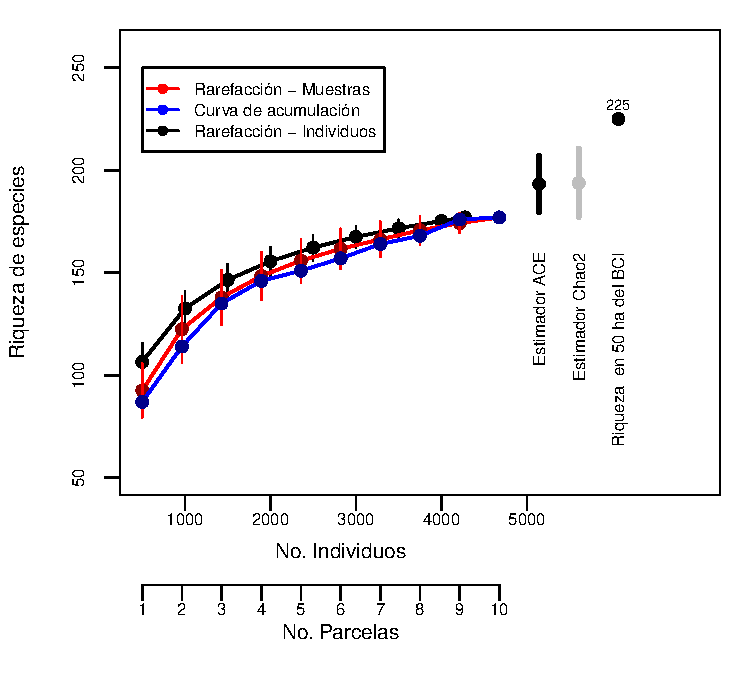
\includegraphics{Alpha-Diversidad_files/figure-latex/rar-1.pdf}
\caption{\label{fig:rar}Curvas de rarefacción basada en individuos y en
muestras de 10 parcelas al azar del BCI. Estimadores de riqueza (ACE) y
Chao2 y riqueza total obtenida en las 50 ha del BCI.}
\end{figure}

En la figura \ref{fig:rar} podemos ver que nuestro muestreo es aceptable
y que aunque no hemos capturado toda la riqueza del área los estimadores
que utilizamos son aceptables. Es posible que en este caso la riqueza de
jacknife sea un mejor estimador. Pero recuerden que normalmente cuando
hacemos un muestreo no tenemos el valor de riqueza total, por lo que no
podemos saber cuan alejados estamos de la realidad.

\chapter{Comparando muestras}\label{comparando-muestras}

Lo que hemos hecho hasta ahora es evaluar nuestro muestreo en general,
como éste se comporta con diferente tamaño de muestras o individuos.
Pero normalmente lo que nos interesa es comparar entre localidades con
diferente condición, seguimos teniendo el problema de que cada parcela
tiene un tamaño distinto, lo que puede afectar a la riqueza.

Para comparar la riqueza necesitamos hacer la rarefacción basada en
individuos, utilizaremos el valor de abundancia de la parcela con menos
individuos. Para esto volvemos a utilizar la función `rarefy´.

\begin{Shaded}
\begin{Highlighting}[]
\NormalTok{R.rar <-}\StringTok{ }\KeywordTok{rarefy}\NormalTok{(BCI_sub, }\KeywordTok{min}\NormalTok{(}\KeywordTok{rowSums}\NormalTok{(BCI_sub)), }\DataTypeTok{se=}\OtherTok{TRUE}\NormalTok{)}
\NormalTok{R.rar}
\end{Highlighting}
\end{Shaded}

\begin{verbatim}
##           31        47        14        20  41        49         48
## S  75.800743 99.301601 94.802702 97.529834 102 88.653177 89.9810001
## se  1.035962  1.499881  1.634561  1.448522   0  1.413692  0.9538244
##           39         26         4
## S  82.343999 90.5559177 87.420264
## se  1.204363  0.6327308  2.222168
## attr(,"Subsample")
## [1] 402
\end{verbatim}

En el objeto \emph{R.rar} tenemos la riqueza interpolada (con
rarefacción) de cada una de las parcelas, el valor utilizado para hacer
la rarefacción es la abundancia de la parcela con menos individuos, en
este caso 402 individuos.

Vamos a generar un gráfico en el cual podamos comparar la riqueza total
de las parcelas del BCI, calcularemos la riqueza de cada parcela con la
función \texttt{specnumber} del paquete \emph{vegan} y la riqueza
estimada con rarefacción con su desviación estándar (Figura
\ref{fig:rpar}).

\begin{Shaded}
\begin{Highlighting}[]
\KeywordTok{par}\NormalTok{(}\DataTypeTok{mfcol=}\KeywordTok{c}\NormalTok{(}\DecValTok{2}\NormalTok{,}\DecValTok{1}\NormalTok{), }\DataTypeTok{oma=}\KeywordTok{c}\NormalTok{(}\DecValTok{2}\NormalTok{,}\DecValTok{1}\NormalTok{,}\DecValTok{1}\NormalTok{,}\DecValTok{1}\NormalTok{), }\DataTypeTok{mar=}\KeywordTok{c}\NormalTok{(}\DecValTok{3}\NormalTok{,}\DecValTok{3}\NormalTok{,}\DecValTok{1}\NormalTok{,}\DecValTok{1}\NormalTok{))}

\NormalTok{Rt<-}\StringTok{ }\KeywordTok{specnumber}\NormalTok{(BCI_sub)}
\KeywordTok{barplot}\NormalTok{(Rt, }\DataTypeTok{ylim=}\KeywordTok{c}\NormalTok{(}\DecValTok{0}\NormalTok{,}\DecValTok{120}\NormalTok{), }\DataTypeTok{col=}\StringTok{"grey30"}\NormalTok{, }\DataTypeTok{cex.main=}\FloatTok{0.8}\NormalTok{,}
         \DataTypeTok{cex.names=}\FloatTok{0.7}\NormalTok{, }\DataTypeTok{cex.axis=}\FloatTok{0.7}\NormalTok{, }\DataTypeTok{mgp=}\KeywordTok{c}\NormalTok{(}\DecValTok{2}\NormalTok{, }\FloatTok{0.35}\NormalTok{, }\DecValTok{0}\NormalTok{))}
\KeywordTok{mtext}\NormalTok{(}\StringTok{"a) Riqueza total por parcela"}\NormalTok{, }\DataTypeTok{side=}\DecValTok{3}\NormalTok{, }\DataTypeTok{cex=}\FloatTok{0.8}\NormalTok{)}
\KeywordTok{mtext}\NormalTok{(}\StringTok{"Número de especies"}\NormalTok{, }\DataTypeTok{side =}\DecValTok{2}\NormalTok{, }\DataTypeTok{at=}\DecValTok{0}\NormalTok{, }\DataTypeTok{line=}\DecValTok{2}\NormalTok{, }\DataTypeTok{cex=}\FloatTok{0.8}\NormalTok{)}

\NormalTok{x<-(}\KeywordTok{barplot}\NormalTok{(R.rar[}\DecValTok{1}\NormalTok{,], }\DataTypeTok{ylim=}\KeywordTok{c}\NormalTok{(}\DecValTok{0}\NormalTok{,}\DecValTok{120}\NormalTok{), }\DataTypeTok{col=}\StringTok{"grey30"}\NormalTok{, }
            \DataTypeTok{cex.main=}\FloatTok{0.8}\NormalTok{, }\DataTypeTok{cex.axis=}\FloatTok{0.7}\NormalTok{, }\DataTypeTok{cex.names=}\FloatTok{0.7}\NormalTok{, }\DataTypeTok{mgp=}\KeywordTok{c}\NormalTok{(}\DecValTok{2}\NormalTok{, }\FloatTok{0.35}\NormalTok{, }\DecValTok{0}\NormalTok{), }
            \DataTypeTok{xlab=}\StringTok{"Sitios"}\NormalTok{, }\DataTypeTok{cex.lab=}\FloatTok{0.8}\NormalTok{))}
\KeywordTok{mtext}\NormalTok{(}\StringTok{"b) Riqueza con rarefacción basada en individuos por parcela"}\NormalTok{, }\DataTypeTok{side =}\DecValTok{3}\NormalTok{, }\DataTypeTok{cex=}\FloatTok{0.8}\NormalTok{)}

\KeywordTok{arrows}\NormalTok{(x,R.rar[}\DecValTok{1}\NormalTok{,] -}\StringTok{ }\DecValTok{2} \NormalTok{*}\StringTok{ }\NormalTok{R.rar[}\DecValTok{2}\NormalTok{,], x,R.rar[}\DecValTok{1}\NormalTok{,] +}\StringTok{ }\DecValTok{2} \NormalTok{*}\StringTok{ }\NormalTok{R.rar[}\DecValTok{2}\NormalTok{,], }\DataTypeTok{length=}\FloatTok{0.05}\NormalTok{,}\DataTypeTok{angle=}\DecValTok{90}\NormalTok{,}\DataTypeTok{code=}\DecValTok{3}\NormalTok{)}
\end{Highlighting}
\end{Shaded}

\begin{figure}[htbp]
\centering
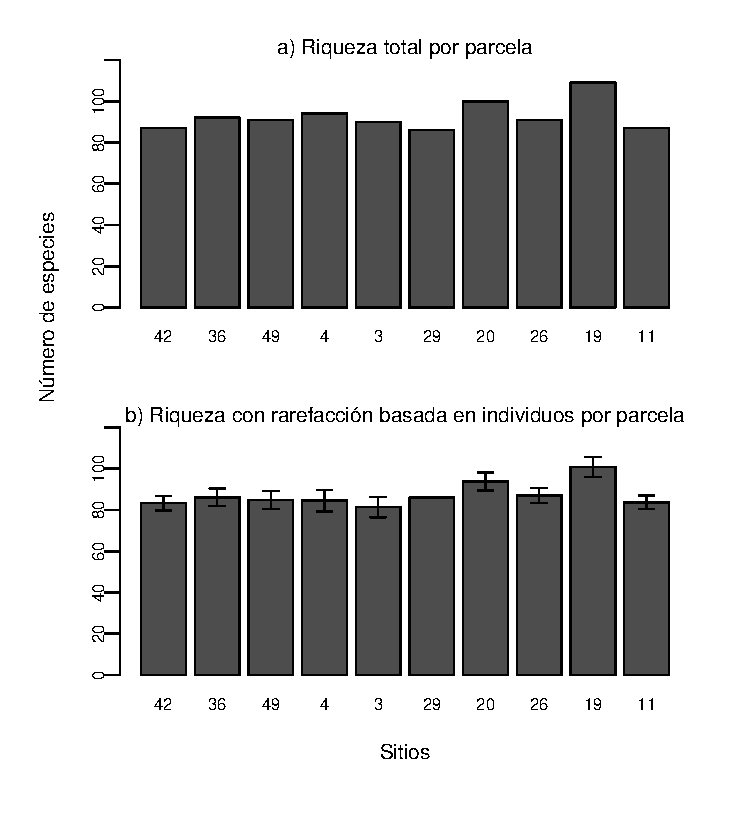
\includegraphics{Alpha-Diversidad_files/figure-latex/rpar-1.pdf}
\caption{\label{fig:rpar}Comparación entre medidas de a. riqueza observada y
b. riqueza obtenida en base a rarefacción con su desviación estándar.}
\end{figure}

Como podemos ver en la figura \ref{fig:rpar}, al comparar la riqueza
entre las diferentes parcelas el patrón se mantiene entre los datos
reales y los datos de la rarefacción, sin embargo, en algunos casos las
diferencias se hacen más evidentes. Y las conclusiones que podemos
obtener son más sólidas.

\chapter{Medidas de Diversidad}\label{medidas-de-diversidad}

Una de las propiedades de las comunidades es la riqueza de especies, sin
embargo, esta medida únicamente nos muestra una de las propiedades de la
comunidad. Una descripción más completa de la comunidad debería incluir
la abundancia de las especies y el número de especies (la riqueza).

Una de las formas más sencillas es desarrollar un modelo de rango de
abundancia u obtener una medida de diversidad, un índice de diversidad.

\section{Modelos de abundancia de
especies}\label{modelos-de-abundancia-de-especies}

El paquete \emph{vegan} tiene algunas funciones que nos permiten
analizar la relación especies-abundancia, algunos de los más utilizados
son los modelos para la distribución de la abundancia de especies (rango
de especies).

\emph{Diagrama de rango de abundancia}

El diagrama de rango de abundancia de especies nos permite graficar las
abundancias logarítmicas en orden decreciente, o en contra de los rangos
de especies (Whittaker, 1965).

La función \textbf{\emph{radfit}} contiene algunos de los modelos más
populares (Wilson, 1991) los cuales utiliza estimadores de máxima
verosimilitud. Algunos de los ajustes utilizados son Brokenstick,
Preemption, Log-normal, Zipf, Zipf-Mandelbrot. No vamos a profundizar en
estos por ahora pero comentaremos como implementarlos en R. Utilizaremos
la función \emph{radfit} para desarrollar el diagrama de rango de
abundancia. La función \emph{radfit} compara los modelos antes
enumerados con el fin de evaluar el mejor ajuste, se utiliza el criterio
de información de Akaike (AIC) y Bayesianos o de Schwartz (BIC). Estos
se basan en log-verosimilitud, pero penalizados por el número de
parámetros estimados. La pena por parámetro es 2 en la AIC y log S en
BIC.

Vamos a construir dos diagramas para dos parcelas del BCI y para los
datos totales de la parcela de 50ha de BCI.

\begin{Shaded}
\begin{Highlighting}[]
\KeywordTok{library}\NormalTok{(vegan)}
\KeywordTok{data}\NormalTok{(BCI)}

\NormalTok{pA<-}\StringTok{ }\NormalTok{BCI[}\DecValTok{3}\NormalTok{,] }\CommentTok{#escogemos una parcela cualquiera del BCI}
\NormalTok{pB<-}\StringTok{ }\NormalTok{BCI[}\DecValTok{23}\NormalTok{,] }\CommentTok{#otra más}
\NormalTok{pBCI<-}\StringTok{ }\KeywordTok{colSums}\NormalTok{(BCI) }\CommentTok{#Los datos de todo BCI}

\NormalTok{RpA<-}\StringTok{ }\KeywordTok{radfit}\NormalTok{(pA)}
\NormalTok{RpB<-}\StringTok{ }\KeywordTok{radfit}\NormalTok{(pB)}
\NormalTok{RpBCI<-}\StringTok{ }\KeywordTok{radfit}\NormalTok{(pBCI)}

\CommentTok{#¿Qué modelo ajusta mejor (tiene menor AIC)?. }
\CommentTok{#Revise los objetos generados }
\NormalTok{RpA; RpB; RpBCI}
\end{Highlighting}
\end{Shaded}

\begin{verbatim}
## 
## RAD models, family poisson 
## No. of species 90, total abundance 463
## 
##            par1      par2     par3    Deviance AIC      BIC     
## Null                                   86.1127 347.8863 347.8863
## Preemption  0.052303                   58.9295 322.7031 325.2029
## Lognormal   0.94937   1.1957           29.2719 295.0455 300.0451
## Zipf        0.14769  -0.86485          50.1262 315.8997 320.8994
## Mandelbrot  3.9471   -1.705    8.1741   5.7342 273.5077 281.0072
\end{verbatim}

\begin{verbatim}
## 
## RAD models, family poisson 
## No. of species 99, total abundance 340
## 
##            par1      par2     par3    Deviance AIC      BIC     
## Null                                   55.4639 322.9662 322.9662
## Preemption  0.038291                   53.4573 322.9597 325.5548
## Lognormal   0.7158    1.0327           21.9550 293.4574 298.6476
## Zipf        0.11689  -0.77842          20.0961 291.5984 296.7887
## Mandelbrot  0.50968  -1.1574   3.9378   7.4609 280.9632 288.7486
\end{verbatim}

\begin{verbatim}
## 
## RAD models, family poisson 
## No. of species 225, total abundance 21457
## 
##            par1      par2     par3    Deviance AIC      BIC     
## Null                                  10261.14 11387.97 11387.97
## Preemption  0.034063                   3788.38  4917.21  4920.63
## Lognormal   3.3569    1.5738            744.30  1875.13  1881.96
## Zipf        0.14679  -0.94912          4335.50  5466.33  5473.16
## Mandelbrot  17.014   -2.0064   15.048   988.02  2120.85  2131.10
\end{verbatim}

Como podemos ver el modelo que mejor ajusta (con AIC o BIC más bajo) es,
en el caso de la parcela A y B, Mandelbrot y en el caso de los datos
completos de la parcela del BCI es Lognormal. Vamos a graficar estas
funciones para poder observar las tendencias (Figura \ref{fig:diag}).

\begin{Shaded}
\begin{Highlighting}[]
\KeywordTok{par}\NormalTok{(}\DataTypeTok{mfcol=}\KeywordTok{c}\NormalTok{(}\DecValTok{1}\NormalTok{,}\DecValTok{3}\NormalTok{))}

\KeywordTok{plot}\NormalTok{(RpA$models$Mandelbrot, }\DataTypeTok{xlim=}\KeywordTok{c}\NormalTok{(}\DecValTok{0}\NormalTok{,}\DecValTok{250}\NormalTok{), }\DataTypeTok{pch=}\DecValTok{19}\NormalTok{, }\DataTypeTok{col=}\StringTok{"black"}\NormalTok{, }\DataTypeTok{cex=}\FloatTok{0.6}\NormalTok{)}
\KeywordTok{plot}\NormalTok{(RpB$models$Mandelbrot, }\DataTypeTok{xlim=}\KeywordTok{c}\NormalTok{(}\DecValTok{0}\NormalTok{,}\DecValTok{250}\NormalTok{), }\DataTypeTok{pch=}\DecValTok{19}\NormalTok{, }\DataTypeTok{col=}\StringTok{"black"}\NormalTok{, }\DataTypeTok{cex=}\FloatTok{0.6}\NormalTok{)}
\KeywordTok{plot}\NormalTok{(RpBCI$models$Lognormal, }\DataTypeTok{xlim=}\KeywordTok{c}\NormalTok{(}\DecValTok{0}\NormalTok{,}\DecValTok{250}\NormalTok{), }\DataTypeTok{pch=}\DecValTok{19}\NormalTok{, }\DataTypeTok{col=}\StringTok{"black"}\NormalTok{, }\DataTypeTok{cex=}\FloatTok{0.6}\NormalTok{)}
\end{Highlighting}
\end{Shaded}

\begin{figure}[htbp]
\centering
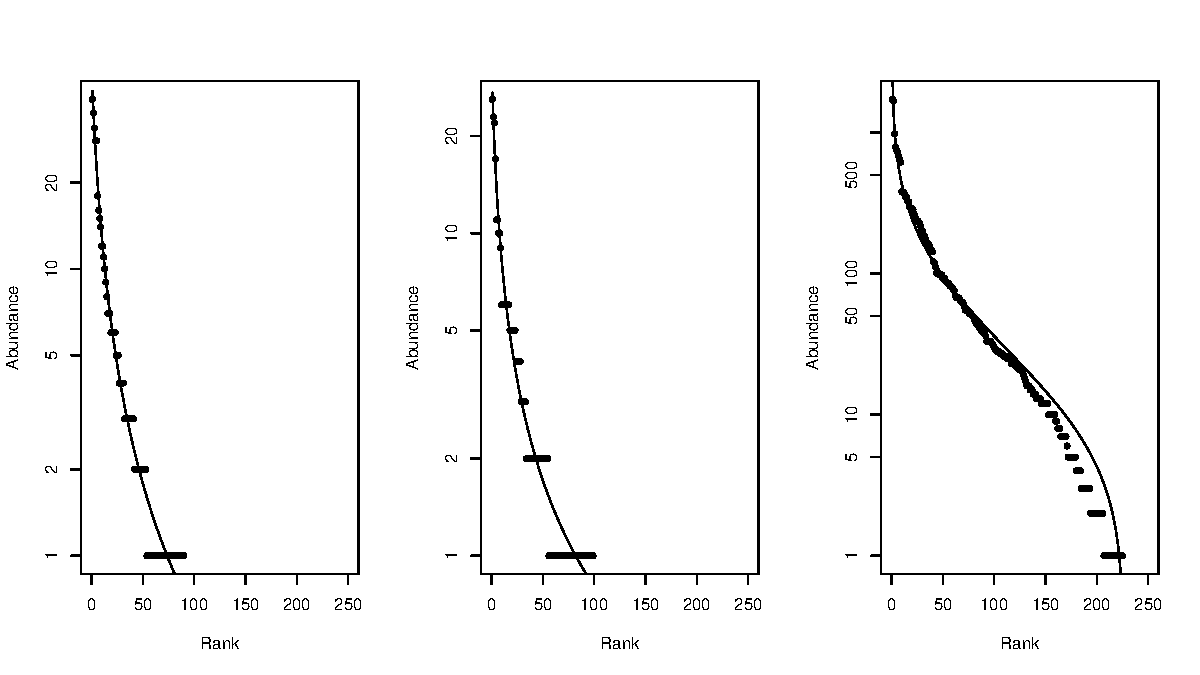
\includegraphics{Alpha-Diversidad_files/figure-latex/diag-1.pdf}
\caption{\label{fig:diag}Rangos de abundancia de dos parcelas de BCI y del
total de parcelas.}
\end{figure}

\section{Índices de Diversidad}\label{indices-de-diversidad}

Los índices de diversidad son considerados como medidas de la varianza
de la distribución de la abundancia de especies. Existen muchos índices
desarrollados aunque seguramente el índice de Simpson y de Shannon son
los más utilizados.

\subsection{Índice de Simpson}\label{indice-de-simpson}

El índice de Simpson \emph{(D)} tiene la tendencia de ser más pequeño
cuando la comunidad es más \emph{diversa}. \emph{D} es interpretado como
la probabilidad de un encuentro intraespecífico, esto quiere decir la
probabilidad de que si tomas dos individuos al azar de la comunidad
ambos sean de la misma especie. Mientras más alta es esta probabilidad
menos diversa es la comunidad (sensu Wallace).

Vamos a ejemplificar para entender este concepto con una comunidad
completamente equitativa, con 10 especies cada una de las cuales tiene
una abundancia de 5.

\begin{Shaded}
\begin{Highlighting}[]
\CommentTok{#Generamos un vector con 10 especies, cada una con 5 individuos}
\NormalTok{abun<-}\StringTok{ }\KeywordTok{rep}\NormalTok{(}\DecValTok{5}\NormalTok{,}\DecValTok{10}\NormalTok{)}

\CommentTok{#Sacamos la abundancia relativa}
\NormalTok{rel<-}\StringTok{ }\NormalTok{abun/}\KeywordTok{sum}\NormalTok{(abun)}
\NormalTok{rel}
\end{Highlighting}
\end{Shaded}

\begin{verbatim}
##  [1] 0.1 0.1 0.1 0.1 0.1 0.1 0.1 0.1 0.1 0.1
\end{verbatim}

A partir de estos datos podemos utilizar el índice de Simpson:

\[
D=\sum_{i=1}^S p_i^2
\]

Donde \emph{S} es el número de especies y \emph{pi} es la proporción de
cada especie.

\begin{Shaded}
\begin{Highlighting}[]
\CommentTok{#calculamos el índice de Simpson}
\NormalTok{D<-}\StringTok{ }\KeywordTok{sum}\NormalTok{((rel)^}\DecValTok{2}\NormalTok{)}
\NormalTok{D}
\end{Highlighting}
\end{Shaded}

\begin{verbatim}
## [1] 0.1
\end{verbatim}

Para evidenciar como \emph{D} (la probabilidad de un encuentro
intraespecífico) aumenta cuando la comunidad es menos equitativa piensa
en el ejemplo de una comunidad con una especie diez veces más abundante
que las demás.

\begin{Shaded}
\begin{Highlighting}[]
\CommentTok{#Generamos un vector con 10 especies, 1 con 50 individuos y el resto con 5 individuos}
\NormalTok{abun2<-}\StringTok{ }\KeywordTok{rep}\NormalTok{(}\KeywordTok{c}\NormalTok{(}\DecValTok{50}\NormalTok{,}\DecValTok{5}\NormalTok{),}\KeywordTok{c}\NormalTok{(}\DecValTok{1}\NormalTok{,}\DecValTok{9}\NormalTok{))}
\CommentTok{#Sacamos la abundancia relativa}
\NormalTok{rel2<-}\StringTok{ }\NormalTok{abun2/}\KeywordTok{sum}\NormalTok{(abun2)}
\NormalTok{rel2}
\end{Highlighting}
\end{Shaded}

\begin{verbatim}
##  [1] 0.52631579 0.05263158 0.05263158 0.05263158 0.05263158 0.05263158
##  [7] 0.05263158 0.05263158 0.05263158 0.05263158
\end{verbatim}

\begin{Shaded}
\begin{Highlighting}[]
\NormalTok{D2<-}\StringTok{ }\KeywordTok{sum}\NormalTok{((rel2)^}\DecValTok{2}\NormalTok{)}
\NormalTok{D2;D}
\end{Highlighting}
\end{Shaded}

\begin{verbatim}
## [1] 0.3019391
\end{verbatim}

\begin{verbatim}
## [1] 0.1
\end{verbatim}

Dado de que queremos un índice que aumenta con la diversidad en vez de
disminuir, sería mejor si podemos interpretar el índice en una forma
directa. Entonces es común usar el inverso del índice de Simpson

\textbf{\emph{invD=1-D}}

\begin{Shaded}
\begin{Highlighting}[]
\NormalTok{invD<-}\StringTok{ }\DecValTok{1}\NormalTok{-D}
\NormalTok{invD2<-}\StringTok{ }\DecValTok{1}\NormalTok{-D2}
\NormalTok{invD;invD2}
\end{Highlighting}
\end{Shaded}

\begin{verbatim}
## [1] 0.9
\end{verbatim}

\begin{verbatim}
## [1] 0.6980609
\end{verbatim}

Como podemos ver ahora la comunidad con una repartición de la abundancia
más equitativa (D) tiene un índice más alto (invD) que la comunidad con
una especie dominante (D2).

\subsection{El índice de Shannon}\label{el-indice-de-shannon}

El índice de Shannon \emph{H} mide más o menos lo mismo que el índice de
Simpson, sin embargo, su lógica teórica está basada en teoría
informática. Esto hace su interpretación un poco menos intuitiva. Sin ir
a más detalle \emph{H} normalmente toma valores entre 1 y 4.5. Valores
encima de 3 son típicamente interpretados como ``diversos''. Por razones
que no son tan obvias como el caso de Simpson el máximo valor que puede
tomar \emph{H} es el logaritmo de \emph{S} (número de especies),
\emph{ln(S)}. El índice de Shannon-Weaver es expresado como:

\[
H=-\sum_{i=1}^S p_ilog_bp_i
\]

Volveremos a utilizar las comunidades que generamos para testar el
índice de Shannon con el fin de evaluar su comportamiento.

\begin{Shaded}
\begin{Highlighting}[]
\NormalTok{H<-}\StringTok{ }\NormalTok{-}\KeywordTok{sum}\NormalTok{((rel*(}\KeywordTok{log}\NormalTok{(rel))))}
\NormalTok{H2<-}\StringTok{ }\NormalTok{-}\KeywordTok{sum}\NormalTok{((rel2*(}\KeywordTok{log}\NormalTok{(rel2))))}
\NormalTok{H;H2}
\end{Highlighting}
\end{Shaded}

\begin{verbatim}
## [1] 2.302585
\end{verbatim}

\begin{verbatim}
## [1] 1.732552
\end{verbatim}

Al igual que en el caso de Simpson, la comunidad más diversa es la
comunidad con una menor dominancia. En la figura \ref{fig:diver} vemos
como varían los dos índices muestran que la comunidad más dominante
representa el 75\% de la comunidad equitativa según Shannon, mientras
que en Simpson muestra que esta representa el 77\%.

\begin{Shaded}
\begin{Highlighting}[]
\NormalTok{##Vamos a generar un gráfico con los dos índices}
\KeywordTok{par}\NormalTok{(}\DataTypeTok{mar=}\KeywordTok{c}\NormalTok{(}\DecValTok{2}\NormalTok{,}\DecValTok{2}\NormalTok{,}\DecValTok{1}\NormalTok{,}\DecValTok{1}\NormalTok{))}
\NormalTok{div<-}\StringTok{ }\KeywordTok{c}\NormalTok{(invD,invD2,H,H2)}
\KeywordTok{names}\NormalTok{(div)<-}\StringTok{ }\KeywordTok{c}\NormalTok{(}\StringTok{"D"}\NormalTok{,}\StringTok{"D2"}\NormalTok{,}\StringTok{"H"}\NormalTok{,}\StringTok{"H2"}\NormalTok{)}
\KeywordTok{barplot}\NormalTok{(div, }\DataTypeTok{ylim=}\KeywordTok{c}\NormalTok{(}\DecValTok{0}\NormalTok{,}\DecValTok{3}\NormalTok{), }\DataTypeTok{main=}\StringTok{"Variación de la diversidad"}\NormalTok{,}
        \DataTypeTok{cex.main=}\FloatTok{0.8}\NormalTok{, }\DataTypeTok{cex.axis=}\FloatTok{0.7}\NormalTok{, }\DataTypeTok{cex.names=}\FloatTok{0.7}\NormalTok{)}
\end{Highlighting}
\end{Shaded}

\begin{figure}

{\centering 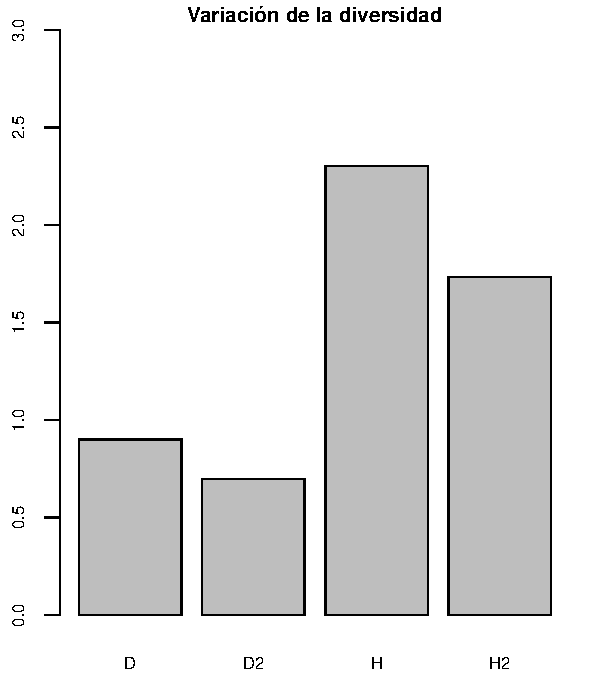
\includegraphics{Alpha-Diversidad_files/figure-latex/diver-1} 

}

\caption{índices de diversidad de Simpson (D y D2)  y de Shannon (H y H2) de dos comunidades con menor y mayor dominancia respectivamente.}\label{fig:diver}
\end{figure}

Aunque como vemos es muy sencillo realizar los índices de Shannon y
Simpson podemos utilizar la función \texttt{diversity} para calcular los
índices.

\begin{Shaded}
\begin{Highlighting}[]
\KeywordTok{diversity}\NormalTok{(abun2, }\StringTok{"simpson"}\NormalTok{)}
\end{Highlighting}
\end{Shaded}

\begin{verbatim}
## [1] 0.6980609
\end{verbatim}

\begin{Shaded}
\begin{Highlighting}[]
\KeywordTok{diversity}\NormalTok{(abun, }\StringTok{"simpson"}\NormalTok{)}
\end{Highlighting}
\end{Shaded}

\begin{verbatim}
## [1] 0.9
\end{verbatim}

\begin{Shaded}
\begin{Highlighting}[]
\KeywordTok{diversity}\NormalTok{(abun, }\StringTok{"shannon"}\NormalTok{)}
\end{Highlighting}
\end{Shaded}

\begin{verbatim}
## [1] 2.302585
\end{verbatim}

\begin{Shaded}
\begin{Highlighting}[]
\KeywordTok{diversity}\NormalTok{(abun2, }\StringTok{"shannon"}\NormalTok{)}
\end{Highlighting}
\end{Shaded}

\begin{verbatim}
## [1] 1.732552
\end{verbatim}

Existen otros índices que pueden ser explorados dentro de la función
\texttt{diversity}.

\chapter{Ejercicio Práctico}\label{ejercicio-practico}

\section{Metodología}\label{metodologia}

En este ejercicio pretendemos estudiar una comunidad de aves a lo largo
de 9 meses del año. Los datos de este trabajo puedes obtenerlos
\href{https://github.com/Ciespinosa/datos_practicas/blob/master/Aves_temporal.xlsx}{aquí}

El objetivo principal de este estudio es entender como las variables
ambientales temperatura y precipitación así como las variables bióticas
(cantidad de frutos e insectos) afectan la riqueza y diversidad de
especies. Adicionalmente, nos interesa determinar si nuestro esfuerzo de
muestreo es suficiente para conocer la riqueza de aves de esta
localidad.

Este trabajo se lo desarrollo en la Reserva Ecológica Arenillas. Tres
localidades separadas 200 metros entre sí fueron seleccionadas. Una vez
por mes se muestrearon las aves utilizando 5 redes de neblina de 9
metros.

\begin{enumerate}
\def\labelenumi{\arabic{enumi}.}
\tightlist
\item
  Con el ejercicio de la comunidad hipotética generada con y sin
  pastoreo.
\end{enumerate}

\begin{enumerate}
\def\labelenumi{\alph{enumi}.}
\tightlist
\item
  Incremente el muestreo a 10 parcelas para cada comunidad (unicamente
  cambie el objeto incrementando las filas y haga el muestreo dos veces
  más).
\item
  Realice una curva de rarefaccion basada en muestras. Se estabiliza la
  curva, es igual en las dos comunidades?
\item
  Obtenga estimadores de riqueza para cada comunidad.
\item
  ¿Cual es el efecto de la diferencia en la densidad de especies sobre
  los resultados?
\end{enumerate}

\begin{enumerate}
\def\labelenumi{\arabic{enumi}.}
\setcounter{enumi}{1}
\tightlist
\item
  Teniendo en cuenta que estamos comparando meses con diferentes
  densidades de individuos. ¿Cómo evaluarías las diferencias en riqueza
  de especies entre meses?
\end{enumerate}

\begin{enumerate}
\def\labelenumi{\alph{enumi}.}
\item
  ¿Cuántos individuos hemos muestreado en cada mes?
\item
\begin{verbatim}
¿Cuántas especies totales hemos detectado en cada mes?
\end{verbatim}
\item
\begin{verbatim}
Explica los resultados del análisis que hayas decidido llevar a cabo.
\end{verbatim}
\end{enumerate}

\begin{enumerate}
\def\labelenumi{\arabic{enumi}.}
\setcounter{enumi}{2}
\tightlist
\item
  Queremos saber si nuestro esfuerzo de muestreo ha sido suficiente para
  caracterizar la diversidad de especies de bosque seco en esta
  localidad y cuál sería en cada caso la riqueza de especies máxima
  esperable. Podríamos ver si el muestreo fue suficiente para la
  estación seca y para la estación lluviosa.
\end{enumerate}

\begin{enumerate}
\def\labelenumi{\alph{enumi}.}
\tightlist
\item
  Calcular la rarefacción basada en individuos y en muestras para el
  bosque en general.
\item
  Hacer un gráfico con las curvas de rarefacción e incluya dos
  estimadores de riqueza.
\item
  Calcular la rarefacción basada en individuos y en muestras para la
  estación seca y lluviosa.
\item
  Hacer un gráfico con las curvas de rarefacción e incluya dos
  estimadores de riqueza para cada estación.
\item
  ¿Qué podemos concluir de este análisis?
\end{enumerate}

\begin{enumerate}
\def\labelenumi{\arabic{enumi}.}
\setcounter{enumi}{3}
\tightlist
\item
  ¿Existen diferencias entre las comunidades de cada mes en cuanto a
  densidad de especies? y en cuanto a equitatividad y diversidad?
\end{enumerate}

\begin{enumerate}
\def\labelenumi{\alph{enumi}.}
\tightlist
\item
  Calcula la riqueza, el índice de equitatividad y diversidad que elijas
  para CADA MUESTRA (mes).
\end{enumerate}

\begin{enumerate}
\def\labelenumi{\arabic{enumi}.}
\setcounter{enumi}{4}
\tightlist
\item
  Los diagramas de rango de abundancia nos da información de la
  equitatividad y la riqueza, tienen patrones de dominancia distintos a
  lo largo de los meses? y entre estaciones?
\end{enumerate}

\begin{enumerate}
\def\labelenumi{\alph{enumi}.}
\tightlist
\item
  Ajusta curvas a cada mes
\item
  Grafica las comunidades con el mejor ajuste y analiza los patrones
  observados.
\item
  Ajusta curvas por cada estación y analiza los resultados.
\end{enumerate}

\begin{enumerate}
\def\labelenumi{\arabic{enumi}.}
\setcounter{enumi}{5}
\tightlist
\item
  Relaciona las variables abióticas y bióticas con los índices evaluados
  utilizando un análisis de correlación de Pearson.
\end{enumerate}

\section{Resultados}\label{resultados}

Organiza la información que ha obtenido de cada uno de estos pasos. Dale
un orden lógico que permita responder la pregunta general planteada.

\section{Conclusiones}\label{conclusiones}

Redacta brevemente las conclusiones que has podido obtener de los
análisis desarrollados.

\bibliography{book}


\end{document}
